\section{Background Research}
\subsection{Temperature Coefficient of Resistance}
The temperature coefficient of resistance (TCR) is a measure of how much the resistance of a material changes with temperature. 

\[TCR = \frac{R-R_0}{R_0(T-T_0)}\]

TCR is defined as the change in resistance per unit change in temperature, usually expressed in parts per million per degree Celsius (ppm/°C) or per Kelvin (ppm/K) \citep{feteira2009negative}.  If the TCR of a material is positive, the material's resistance increases with temperature. If the TCR is negative, then the material's resistance decreases with temperature.

\begin{figure}[H]
    \centering
    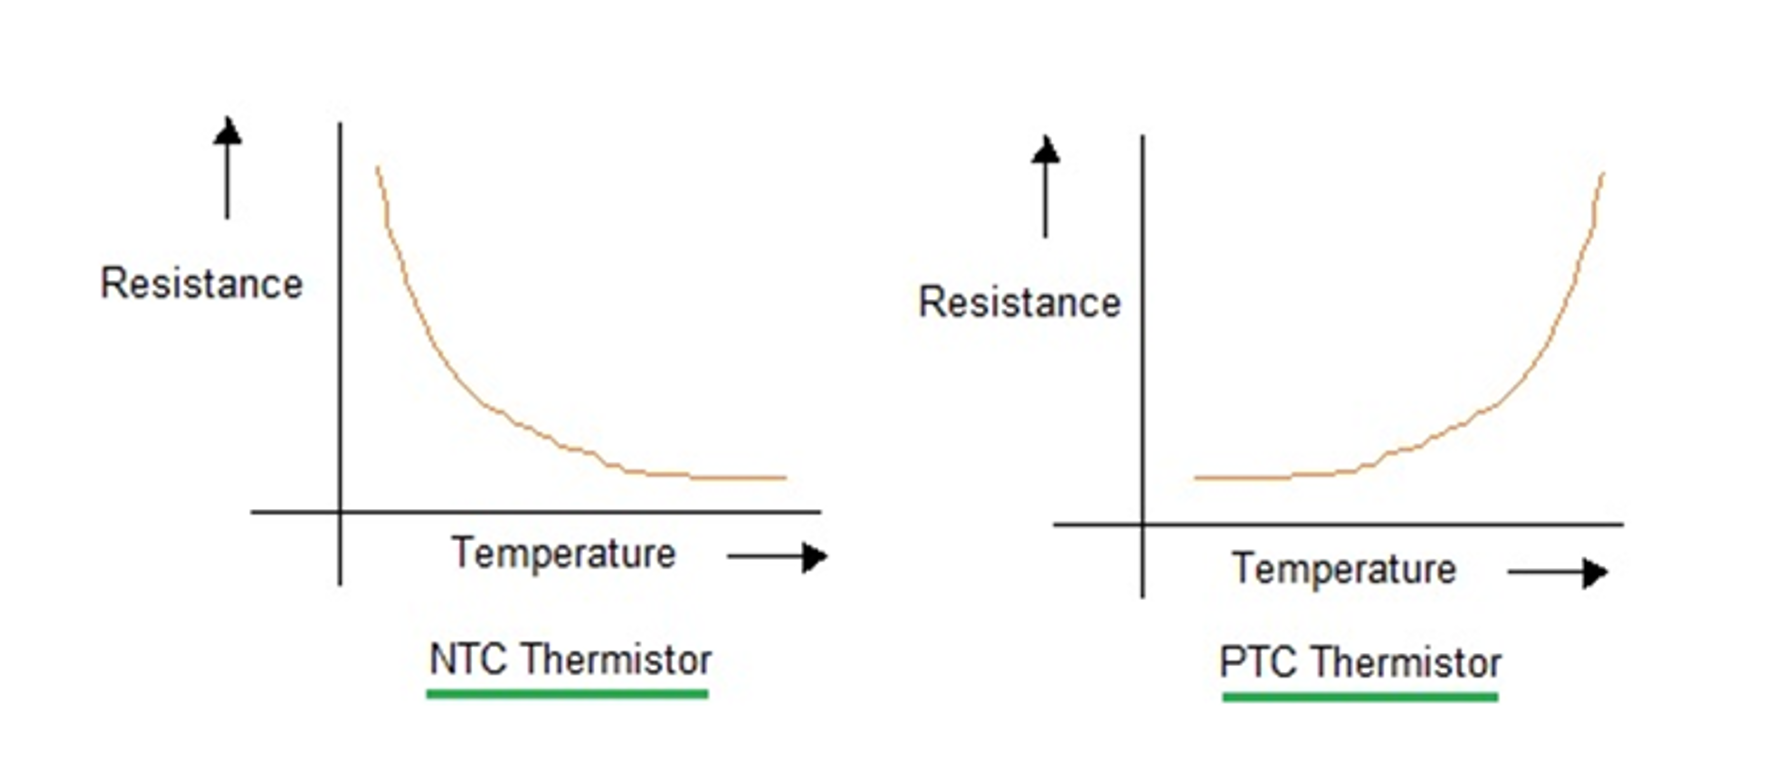
\includegraphics[width=130mm,height=\textheight,keepaspectratio]{images/ntc_ptc.png}
    \caption{Resistance vs Temperature Graph for NTC and PTC Thermistors \citep{amethermptcntc}}
    \label{fig:ntc_ptc}
\end{figure}

\subsection{Conductor - Resistance vs Temperature}
Temperature has a significant effect on the resistance of a regular conductive metallic substance. As the temperature of a metal increases, its resistance also increases. This positive TCR is due to the fact that the increased temperature causes the electrons in the metal to vibrate more and thus collide with each other more often, increasing the resistance \citep{butera1997dependence}. The magnitude of the temperature coefficient of resistance varies from one metal to another, with some metals having a higher coefficient than others.

\subsection{Semiconductor - Resistance vs Temperature}
Temperature impacts the resistance of a semiconductor in two ways. First, as temperature increases, the mobility of the charge carriers in the semiconductor increases, which reduces the resistance of the semiconductor. Second, as temperature increases, more charge carriers are generated, which also reduces the resistance of the semiconductor \citep{butera1997dependence}. Thus, at low temperatures close to absolute zero, the resistance of a semiconductor is very high. The temperature coefficient of resistance (TCR) of a semiconductor is usually negative, meaning that resistance decreases with increasing temperature. The TCR of a semiconductor is dependent on the type of semiconductor material and the doping level.

\begin{figure}[H]
    \centering
    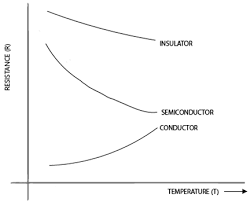
\includegraphics[width=75mm,height=\textheight,keepaspectratio]{images/conductor_semiconductor_insulator.png}
    \caption{Resistivity vs Temperature Graph for Conductors, Semiconductors, and Insulators \citep{mandal_2022}. This plot shows the positive TCR of conductors and the negative TCR for semiconductors and insulators.}
    \label{fig:materials_RT_Plot}
\end{figure}

\section{Hypothesis}
If the temperature of an NTC thermistor increases, then the resistance of the NTC thermistor will decrease exponentially. If the temperature of an NTC thermistor decreases, then the resistance of the NTC thermistor will increase exponentially. 